
\documentclass{beamer}

\usepackage{graphicx}
\usepackage{natbib}
\usepackage{hyperref}
\usepackage{tabularx}
%\usepackage[light]{FiraSans}
\usepackage[british]{datetime2}
\usetheme{default}
\setbeamertemplate{navigation symbols}{} % No navigation symbols
\definecolor{ntnu}{cmyk}{100,75,0,5}
\setbeamercolor{alerted text}{fg=ntnu}
\setbeamercolor{frame title}{fg=ntnu}
\setbeamercolor{title}{fg=ntnu}
\setbeamercolor{subtitle}{fg=ntnu}

\usecolortheme[named=white]{structure} % White titles and such
\setbeamercolor{normal text}{fg=white} % White text
\setbeamercolor{background canvas}{bg=black} % Black background

%\setbeamercovered{transparent}

%\setbeamertemplate{itemize item}{\color{white}$\bullet$} 
% Include above line to remove bullet indicators

\setbeamertemplate{footline}{
\begin{tabularx}{\textwidth} {
	 >{\raggedright\arraybackslash}X 
  	 >{\centering\arraybackslash}X 
  	 >{\centering\arraybackslash}X 
  	 >{\centering\arraybackslash}X 
  	 >{\centering\arraybackslash}X 
  	 >{\centering\arraybackslash}X}
	
	\raisebox{-0.3cm}
	{
\includegraphics[width=2cm, keepaspectratio]{img/ntnu_uten_slagord_neg.pdf}} &
	\insertshortauthor & 
	\insertshorttitle &
	\insertdate &
	\insertsection &
	$\big|$ \insertframenumber
\end{tabularx}
}

\makeatletter
\makeatother

%----------------------------------------------------------------------------------------
%	TITLE PAGE
%----------------------------------------------------------------------------------------

\title[Communal violence]{Precolonial states and communal violence}

\subtitle{}

\author[Wishman]{Marius Swane Wishman} 
\author[Theisen]{Ole Magnus Theisen}
\author[Wishman \& Theisen]{Marius Swane Wishman \inst{$\dagger$} \and Ole
Magnus Theisen \inst{$\ddagger$}}
\institute[]{\inst{$\dagger$} Department of Sociology and Political Science, NTNU \and %
                      \inst{$\ddagger$} Independent PhD researcher}
\date{SecVic presentation} 

\begin{document}

\begin{frame}[plain]
\titlepage 
\centering

\includegraphics[width=5cm]{img/ntnu_uten_slagord_neg.pdf} 
\end{frame}

\section{Communal violence}

\begin{frame}
\frametitle{Communal violence}

\begin{columns}
	\column{.5\textwidth}
\begin{figure}[htpb]
	\centering
	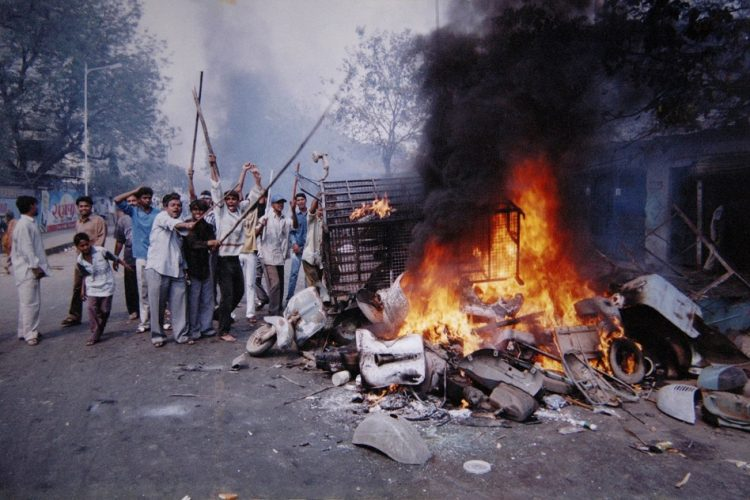
\includegraphics[width=\linewidth]{img/communal-Voilence-750x500.jpg}
	\label{cv}
\end{figure}

	\column{.5\textwidth}

\begin{itemize}
	\item[-] Competition over resources \citep{Detges_2017, D_ring_2020,
		Fjelde2012, van_Weezel_2019, Petrova_2022} \pause
	\item[-] Horizontal inequalities \citep{Fjelde2014} \pause
	\item[-] Historical factors and institutions \citep{Ali_2018, Eck2014,
		Wig2018}
\end{itemize}

\end{columns}

\end{frame}

\begin{frame}
\frametitle{Communal violence in Africa}
\begin{figure}[htpb]
	\centering
	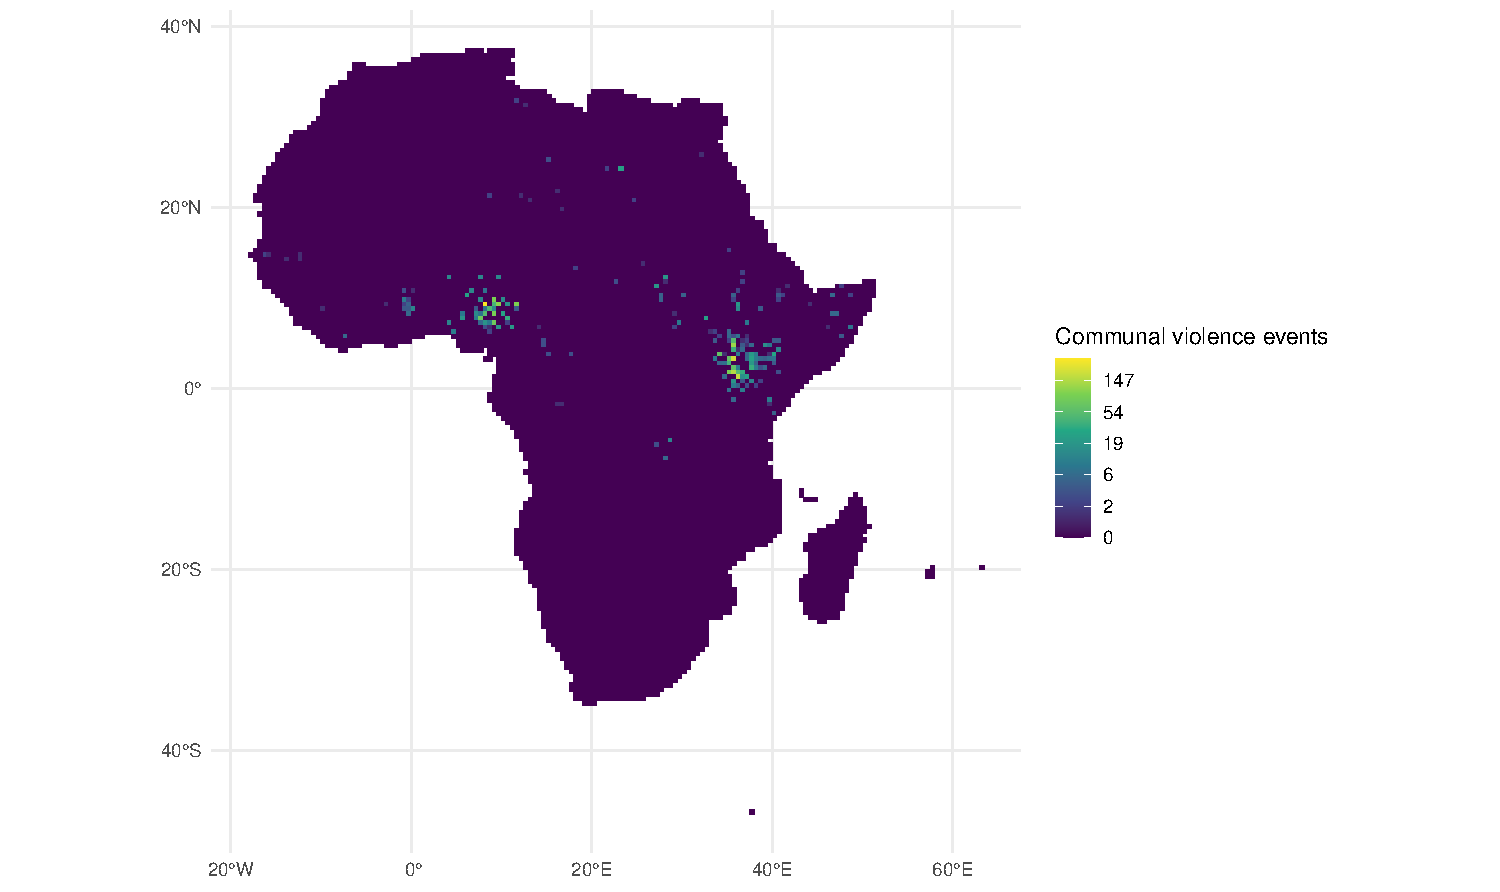
\includegraphics[width=\linewidth]{../R/Output/logOrg3.pdf}
	\caption{Communal violence (log-transformed for visualisation)}
	\label{org3}
\end{figure}
\end{frame}

\section{Peace in the absence of states}

\begin{frame}{Why are communities prone to conflict}

\begin{itemize}
	\item[-] Information problems \pause
		% Individual reputations
		% Individual transgressions lead to collective retribution
	\item[-] Lack of credible commitments \pause
		% Lack of leaders and institutions to make commitments credible
		% by being able to punish spoilers.
		% Lack of overarching authority to prevent the stronger party
		% reneging on agreements.
	\item[-] Security dilemma 
		% The combination of the above make defensive moves look
		% threatening. Chronic uncertainty. Arms races, escalation of
		% posturing and preemptive strikes are the result.
\end{itemize}	

\end{frame}

\begin{frame}{Non-state solutions}

	\begin{itemize}
		\item[-] Fear of feuding \pause
		\item[-] In-group policing \pause
		\item[-] Politeness and hospitality norms
	\end{itemize}

\end{frame}

\begin{frame}{Non-state solutions}

	\begin{block}{}
		Augo du bruke \\
		fyrr inn du gjeng, \\
		i kot og kråom,\\
		i kot og i krokom.\\
		For d'er uvist å vita \\
		kvar uvener sit\\
		fyre din fot.
	\end{block}

\end{frame}

\section{Leviathan}

\begin{frame}{Enter Leviathan}

\begin{figure}[htpb]
	\centering
	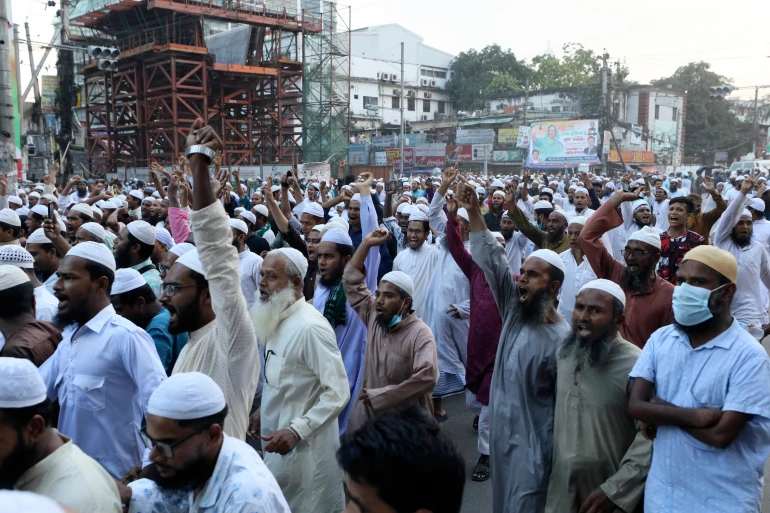
\includegraphics[width=\linewidth]{img/ap.png}
	\caption{Muslims protesting against local Hindu insult to Islam...}%
	\label{ap}
\end{figure}	

\end{frame}

\begin{frame}{Enter Leviathan}

\begin{figure}[htpb]
	\centering
	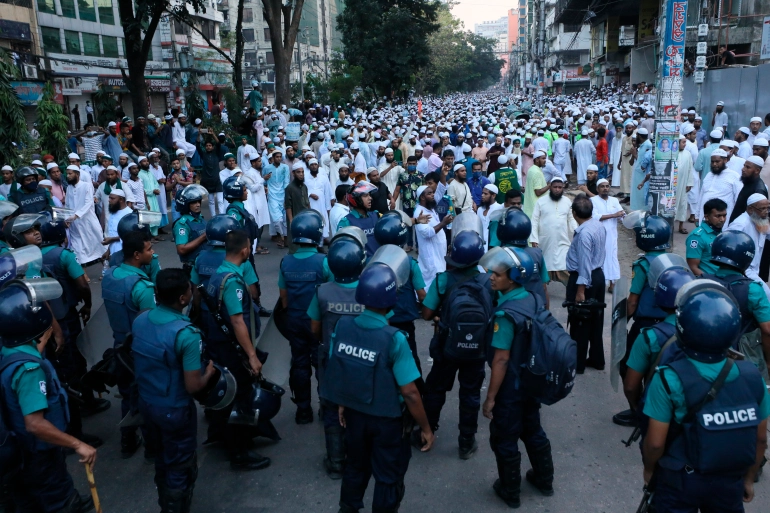
\includegraphics[width=\linewidth]{img/AP.png}
	\caption{...being stopped by police}%
	\label{AP}
\end{figure}	

\end{frame}

\section{Inheritance of precolonial states}

\begin{frame}
\frametitle{Precolonial states} 

\begin{figure}[htpb]
	\centering
	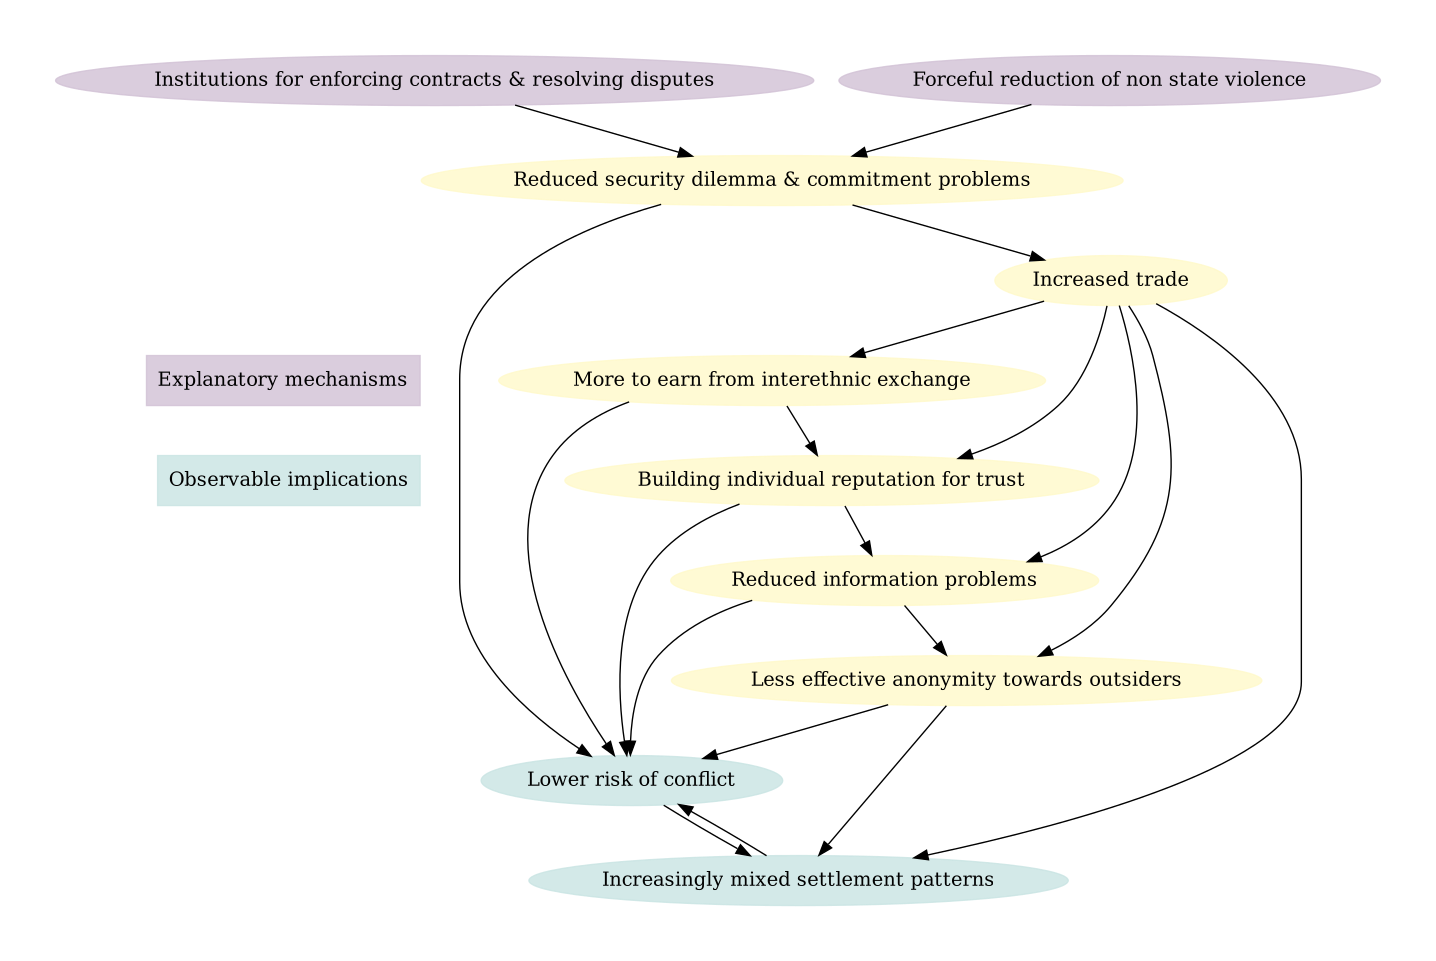
\includegraphics[width=.8\linewidth]{img/OMTcausal.png}
	\caption{Causal diagram}%
	\label{causal}
\end{figure}
\end{frame}

\begin{frame}
\frametitle{Precolonial states} 

\begin{figure}[htpb]
	\centering
	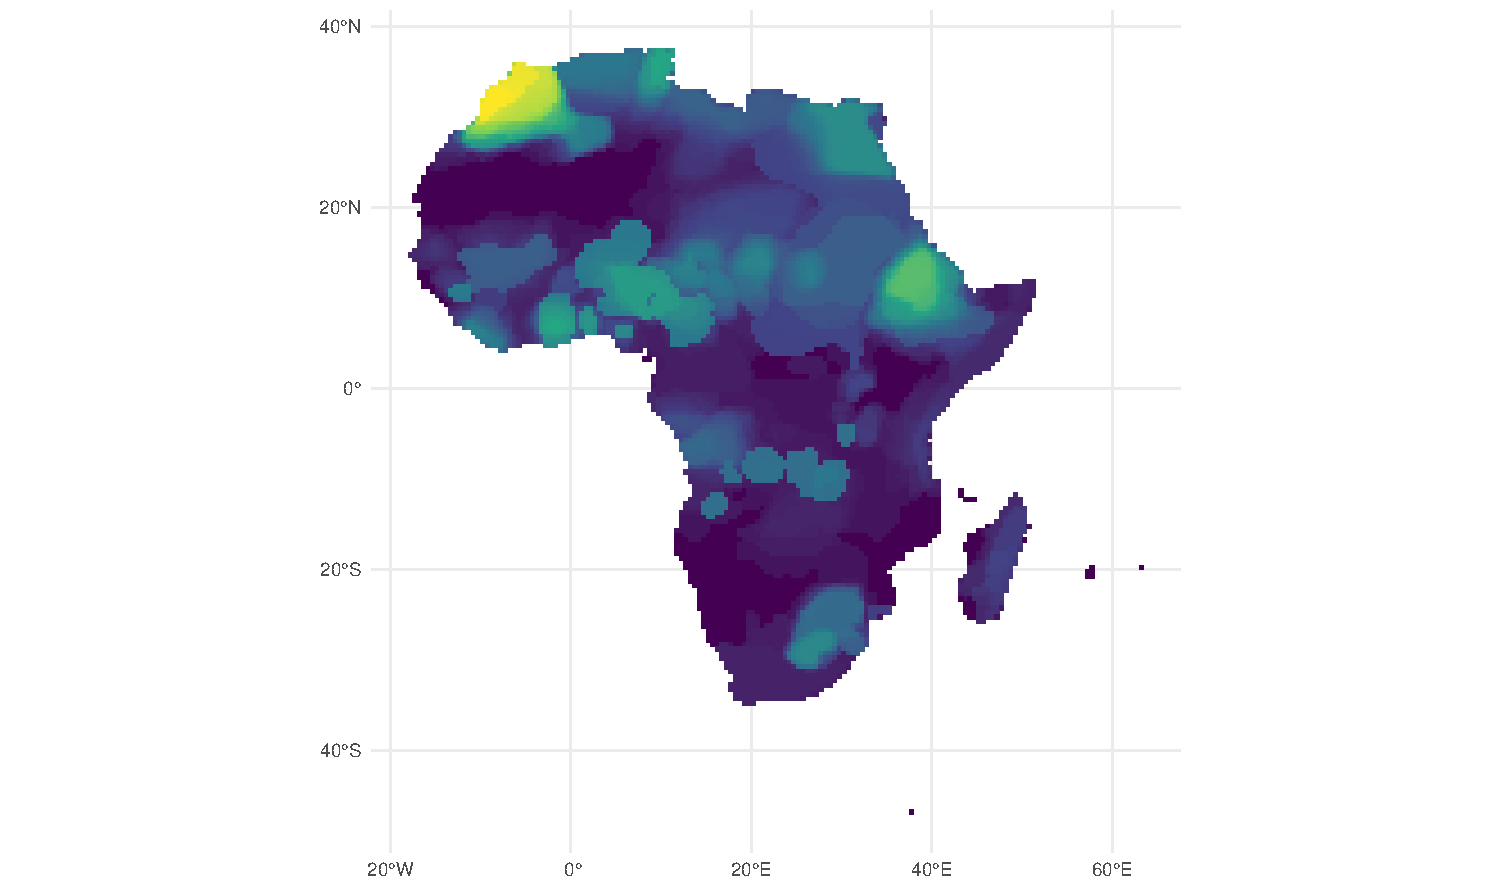
\includegraphics[width=\linewidth]{../R/Output/sqrtSpAll.pdf}
	\caption{Precolonial state presence}%
	\label{sp}
\end{figure}
\end{frame}

\begin{frame}{Precolonial states}
\begin{figure}[htpb]
	\centering
	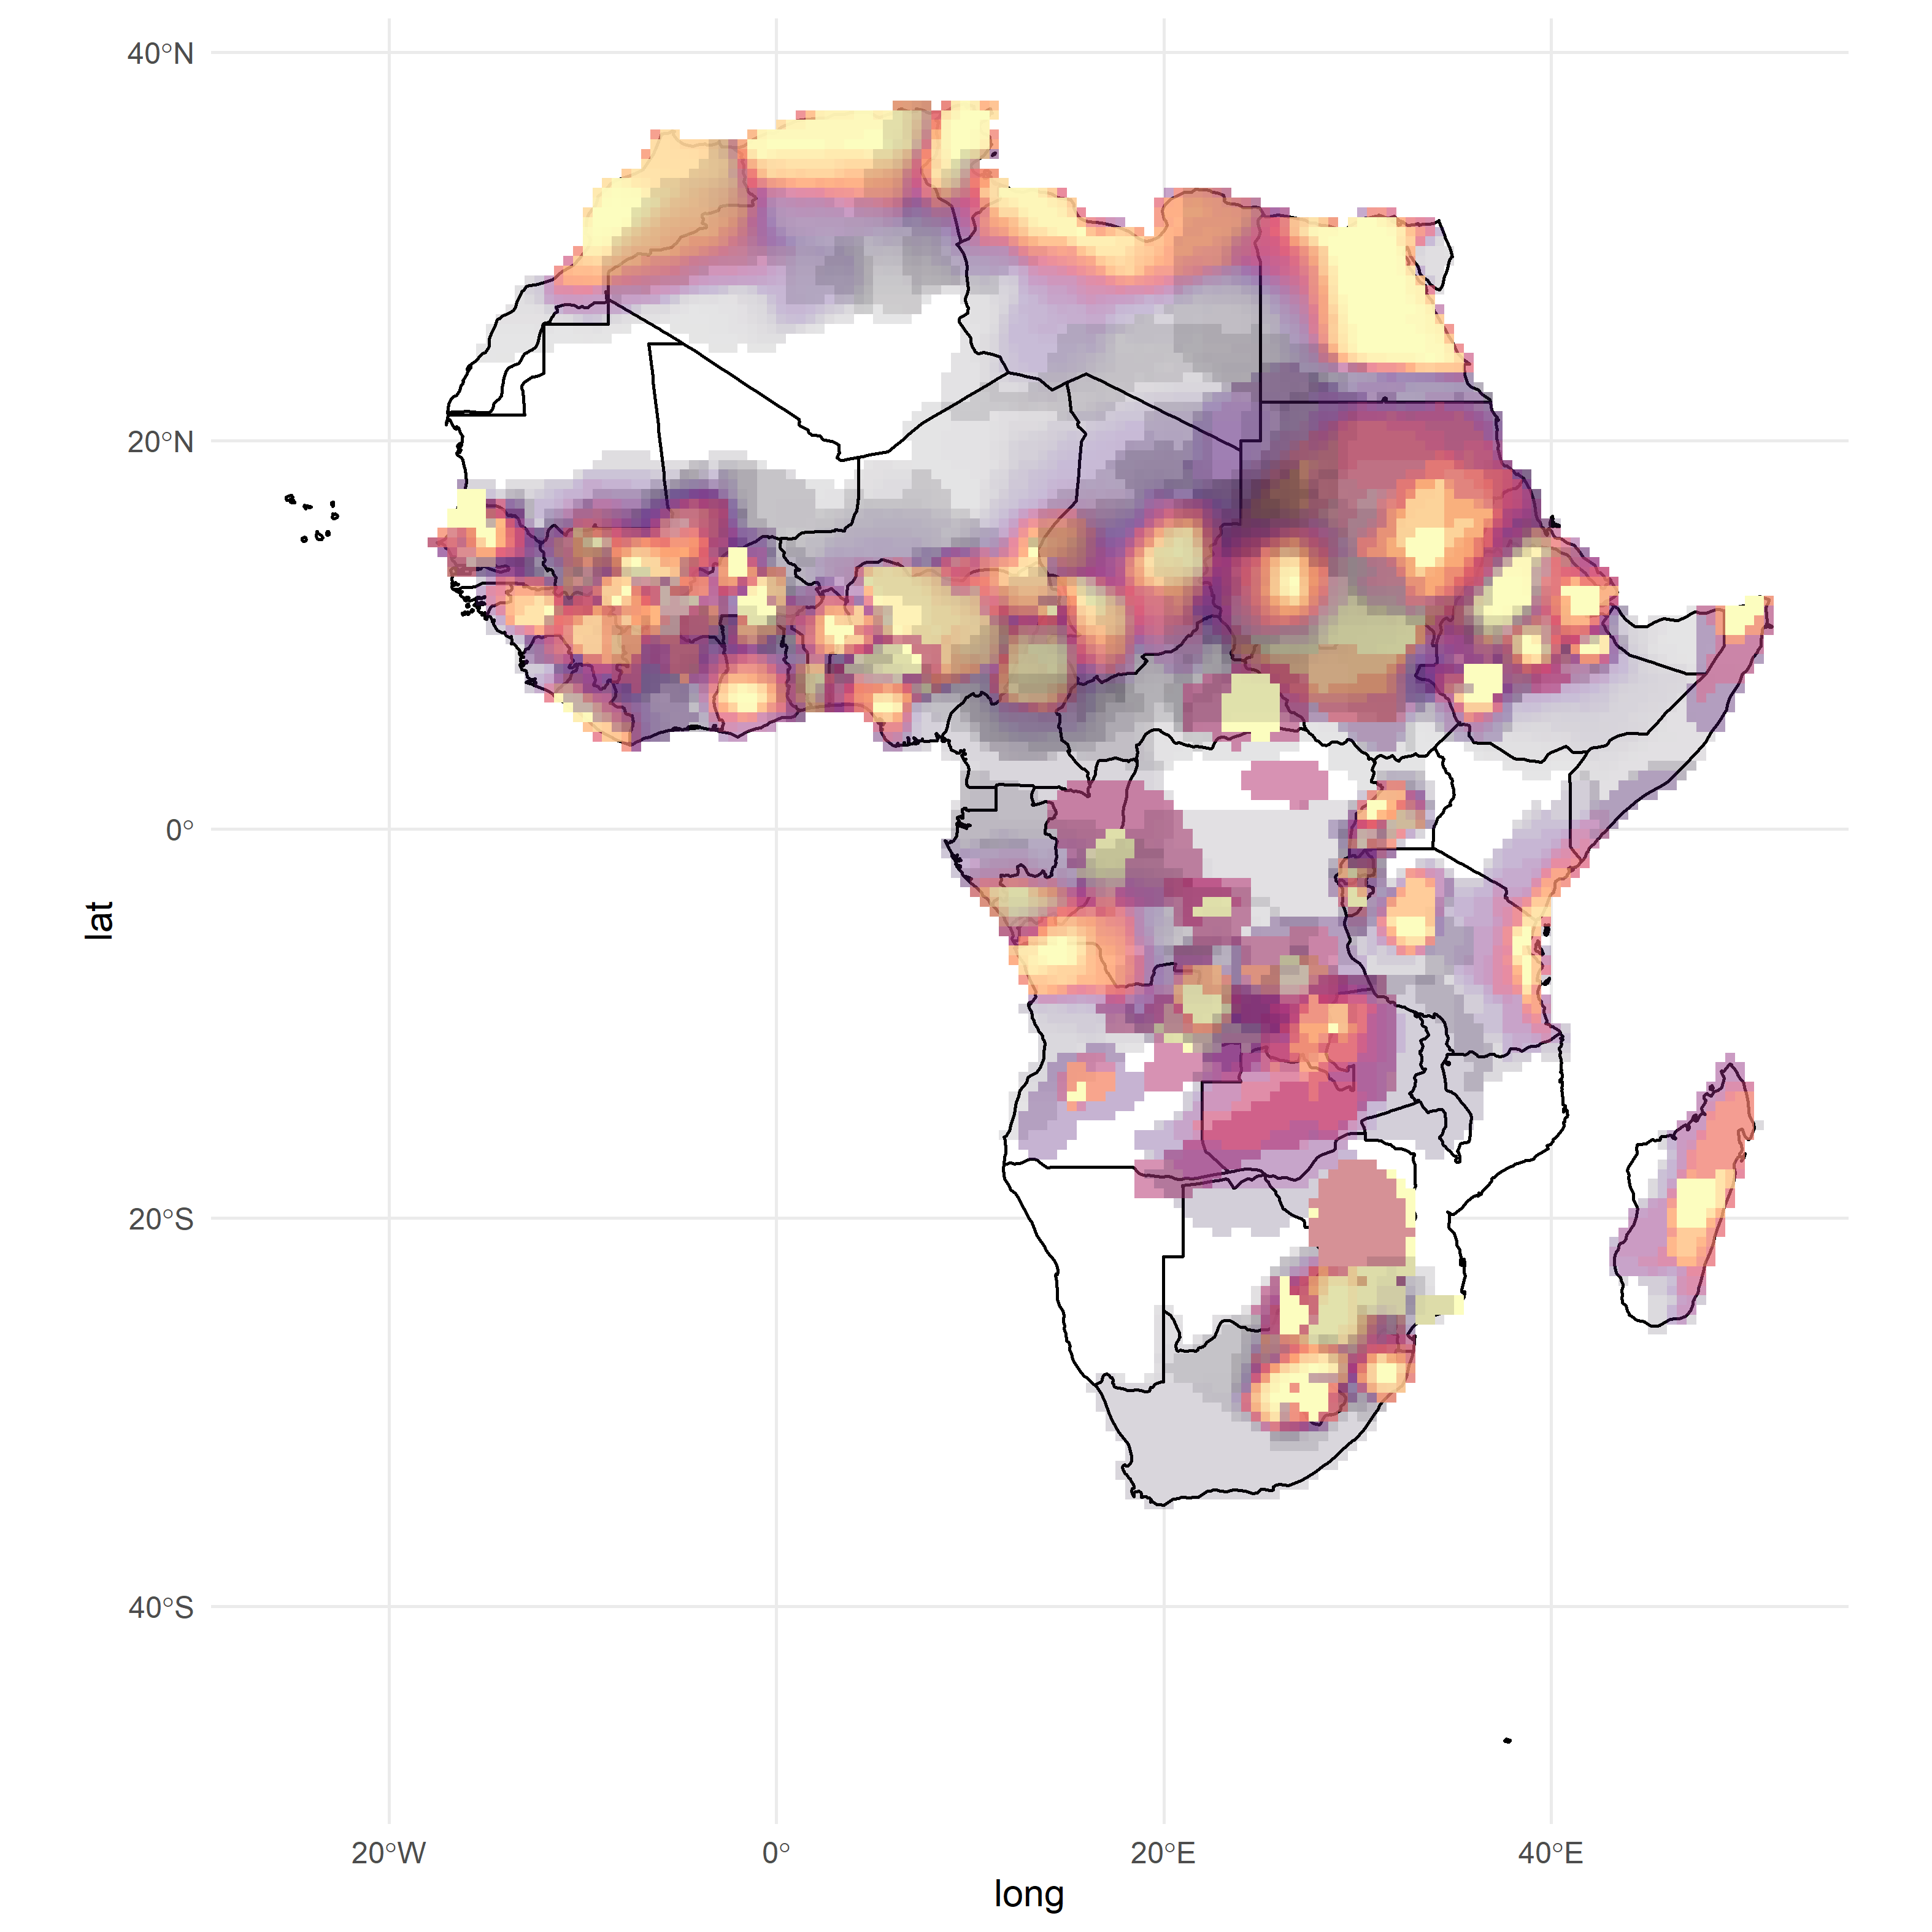
\includegraphics[width=\linewidth]{img/geo_isd_all.png}
	\caption{Precolonial state presence per pre-colonial state}%
\end{figure}
\end{frame}

\begin{frame}{Precolonial states}

	\begin{figure}[htpb]
		\centering
		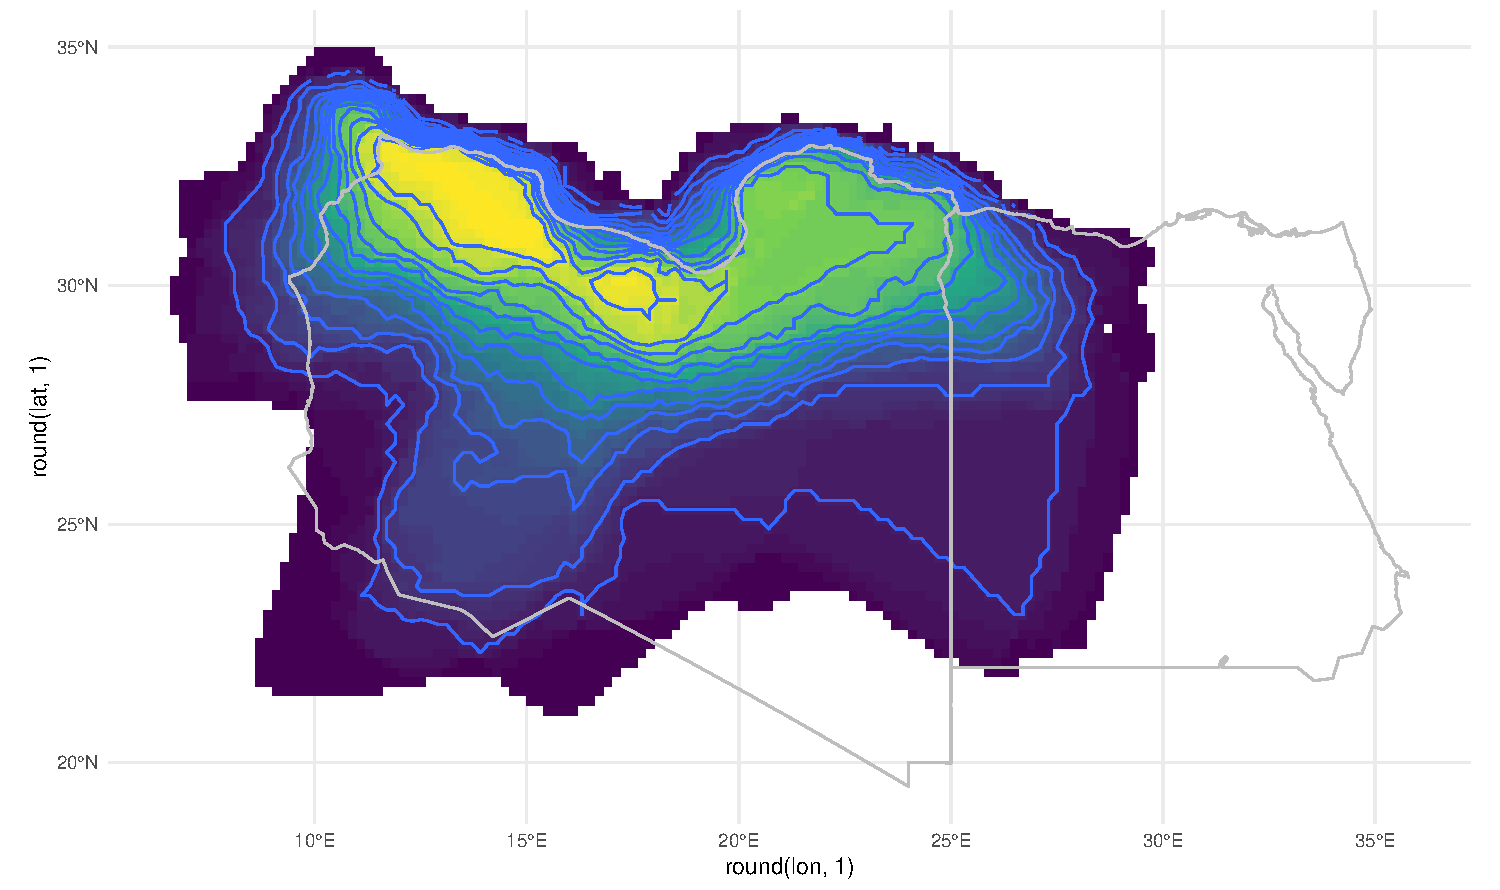
\includegraphics[width=\linewidth]{img/libya.pdf}
	\end{figure}

\end{frame}

\begin{frame}{Colonial states}

\begin{itemize}
	\item[-] The practical nature of colonial regimes \pause 
		% Outside administrative capitals colonial administration relied
		% on EMPOWERING existing local rulers.
	\item[-] Institutions persist \pause
	\item[-] Inter-ethnic traditions of trade and interaction
\end{itemize}	

\end{frame}

\section{Results}

\begin{frame}{Main results}

	\begin{figure}[htpb]
		\centering
		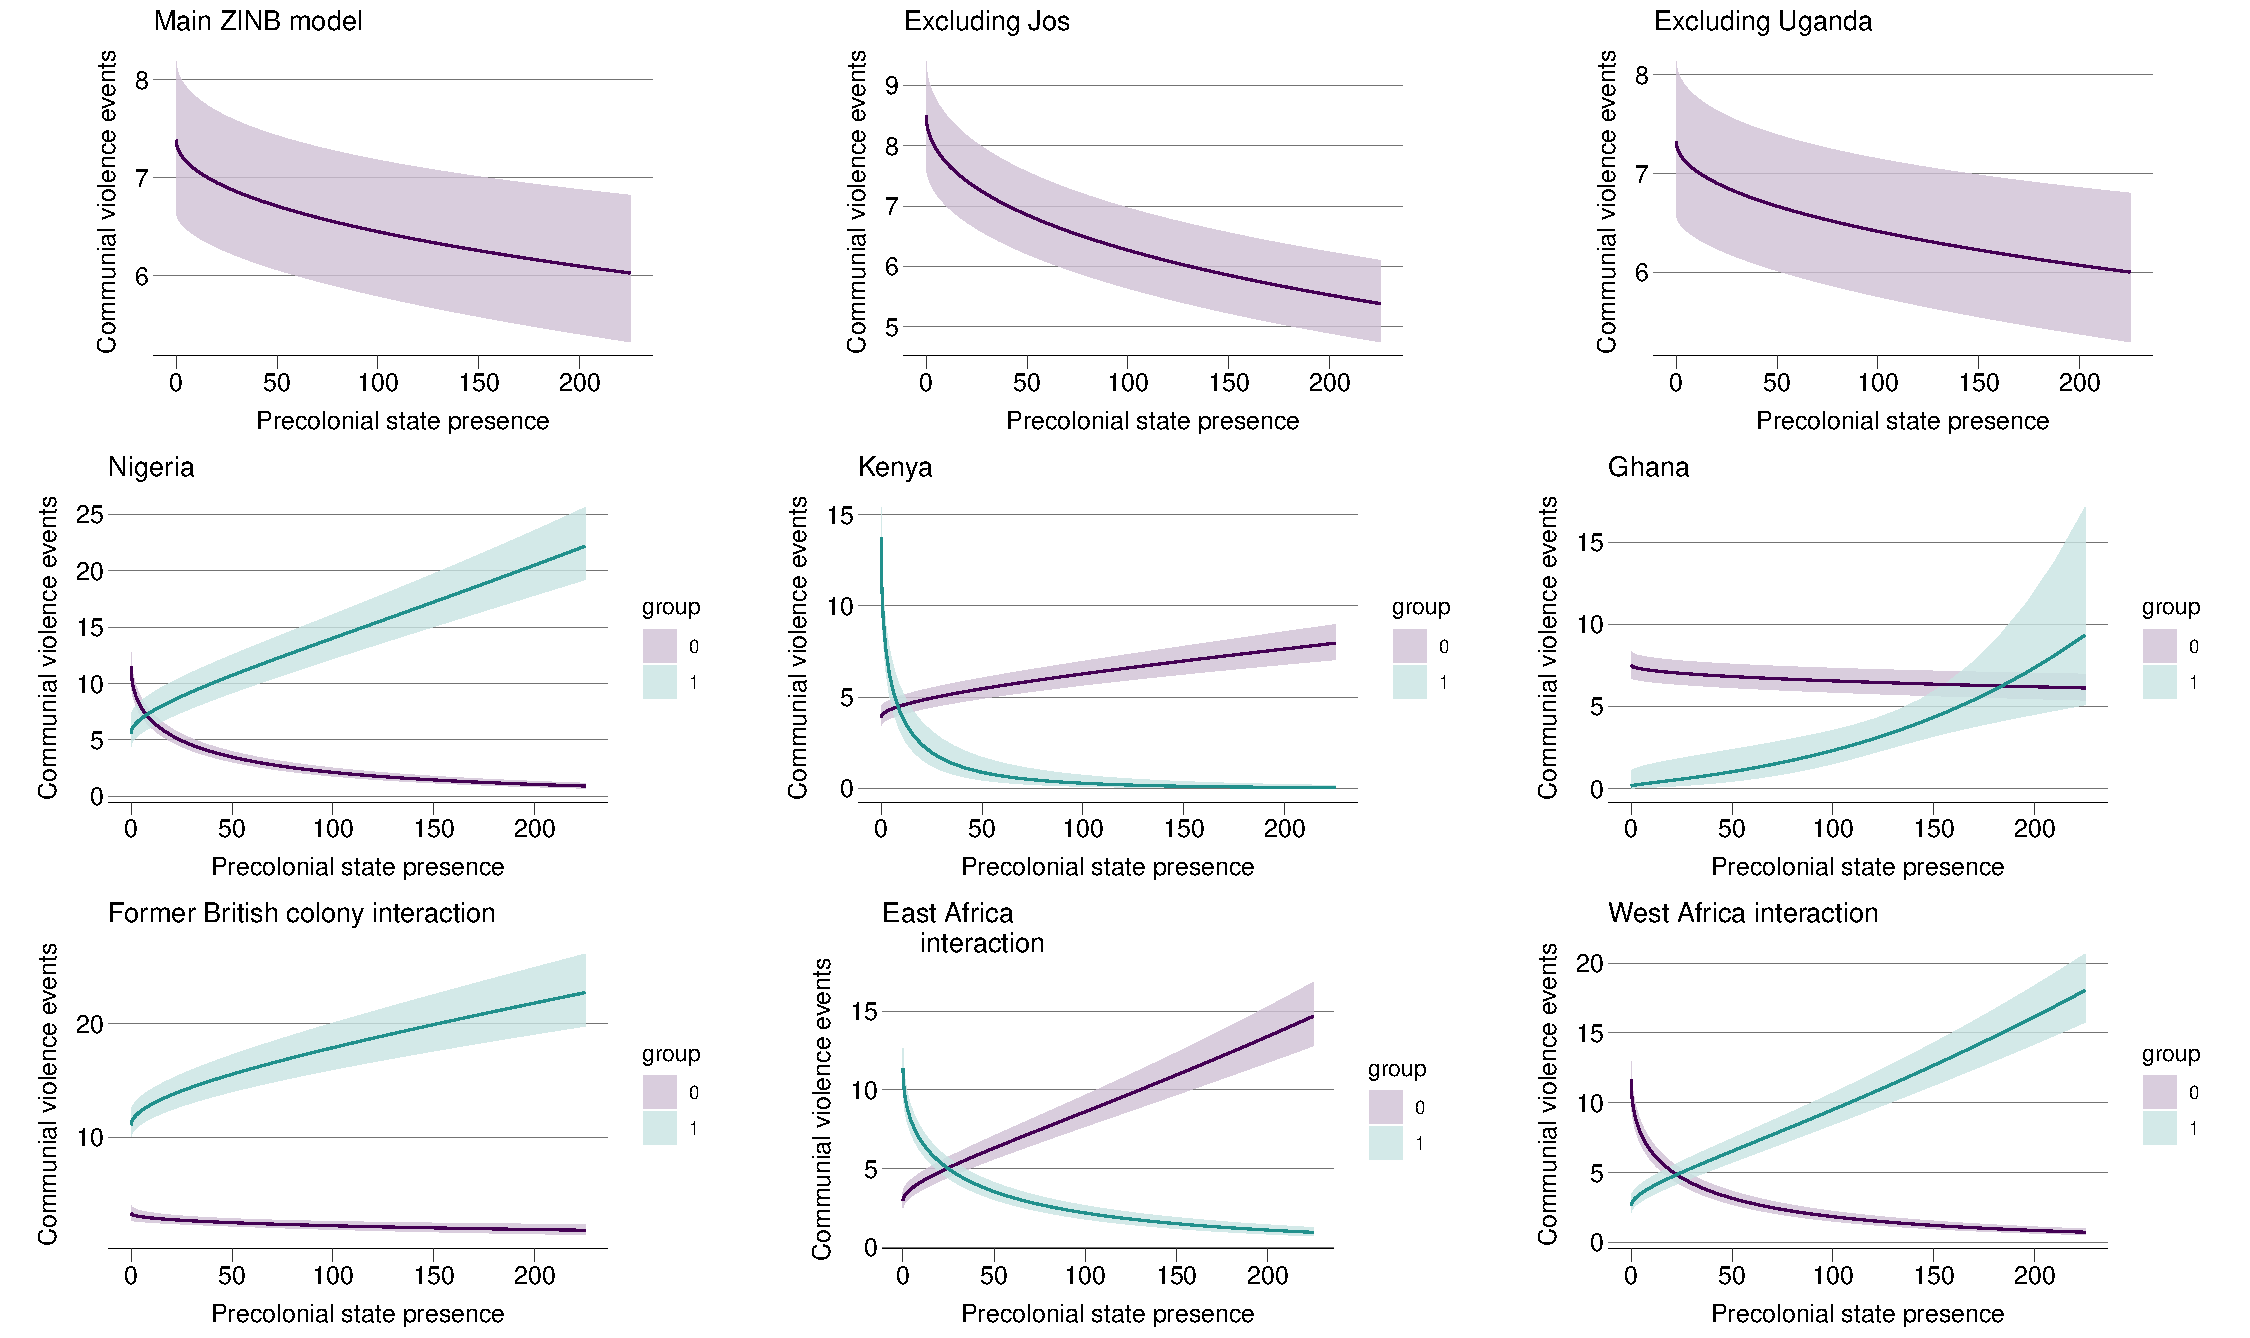
\includegraphics[width=\linewidth]{img/org3plots.pdf}
	\end{figure}

\end{frame}

\begin{frame}{East African phenomenon? Or just Nigeria?}

	\begin{figure}[htpb]
		\centering
		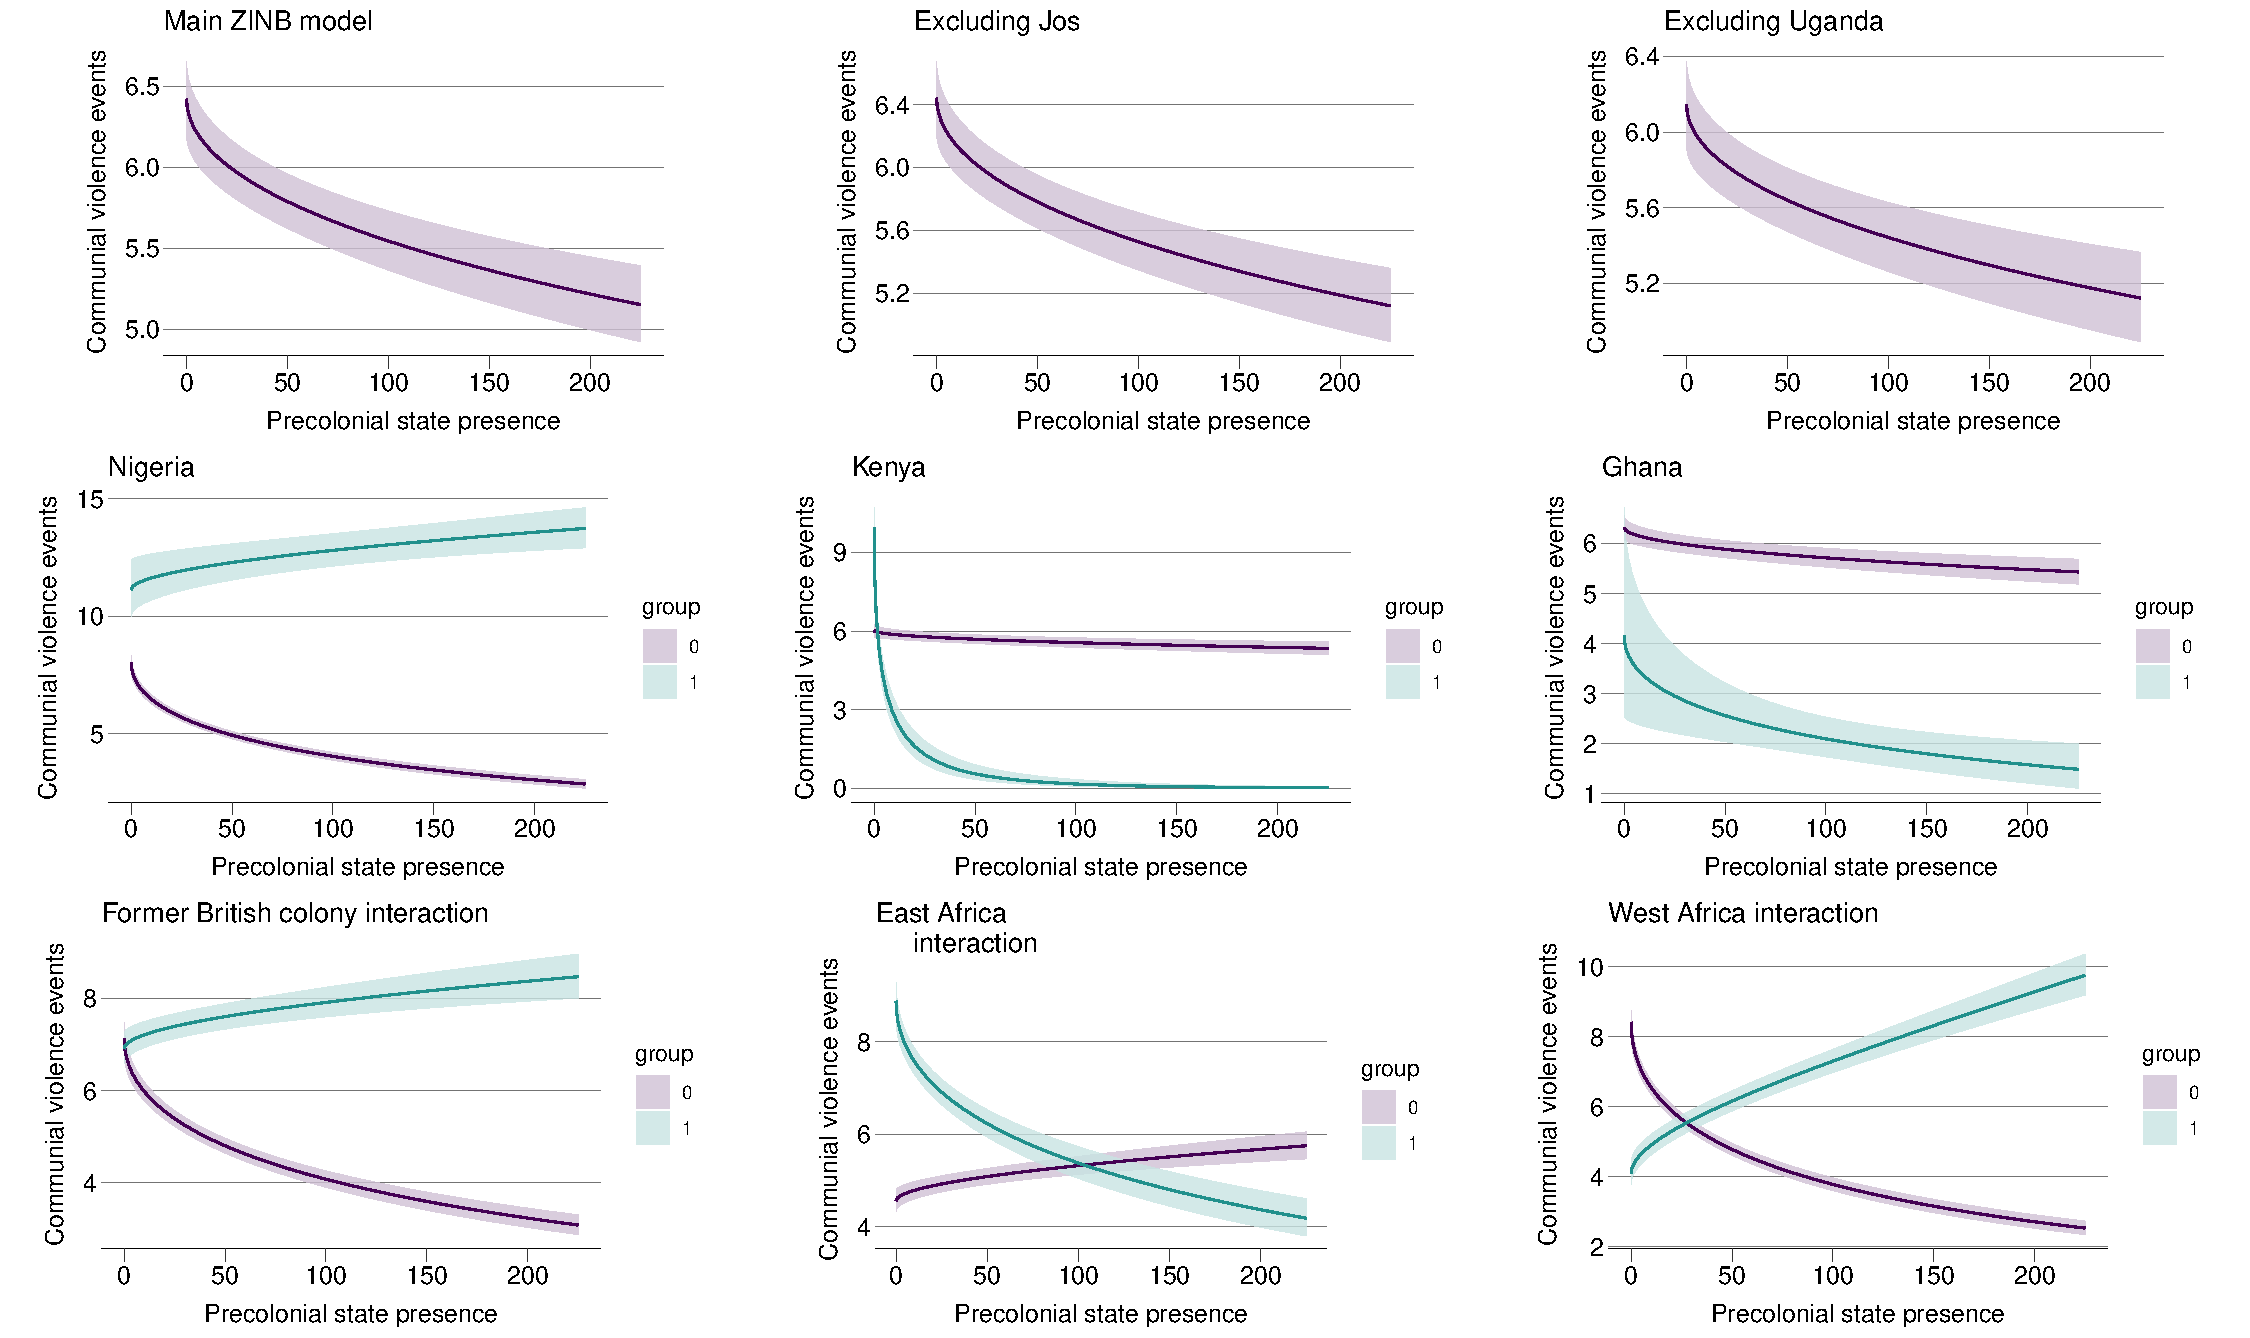
\includegraphics[width=\linewidth]{img/acledplots.pdf}
	\end{figure}	

\end{frame}
\section{Settlement patterns}

\begin{frame}{Settlement patterns}

	\begin{figure}[htpb]
		\centering
		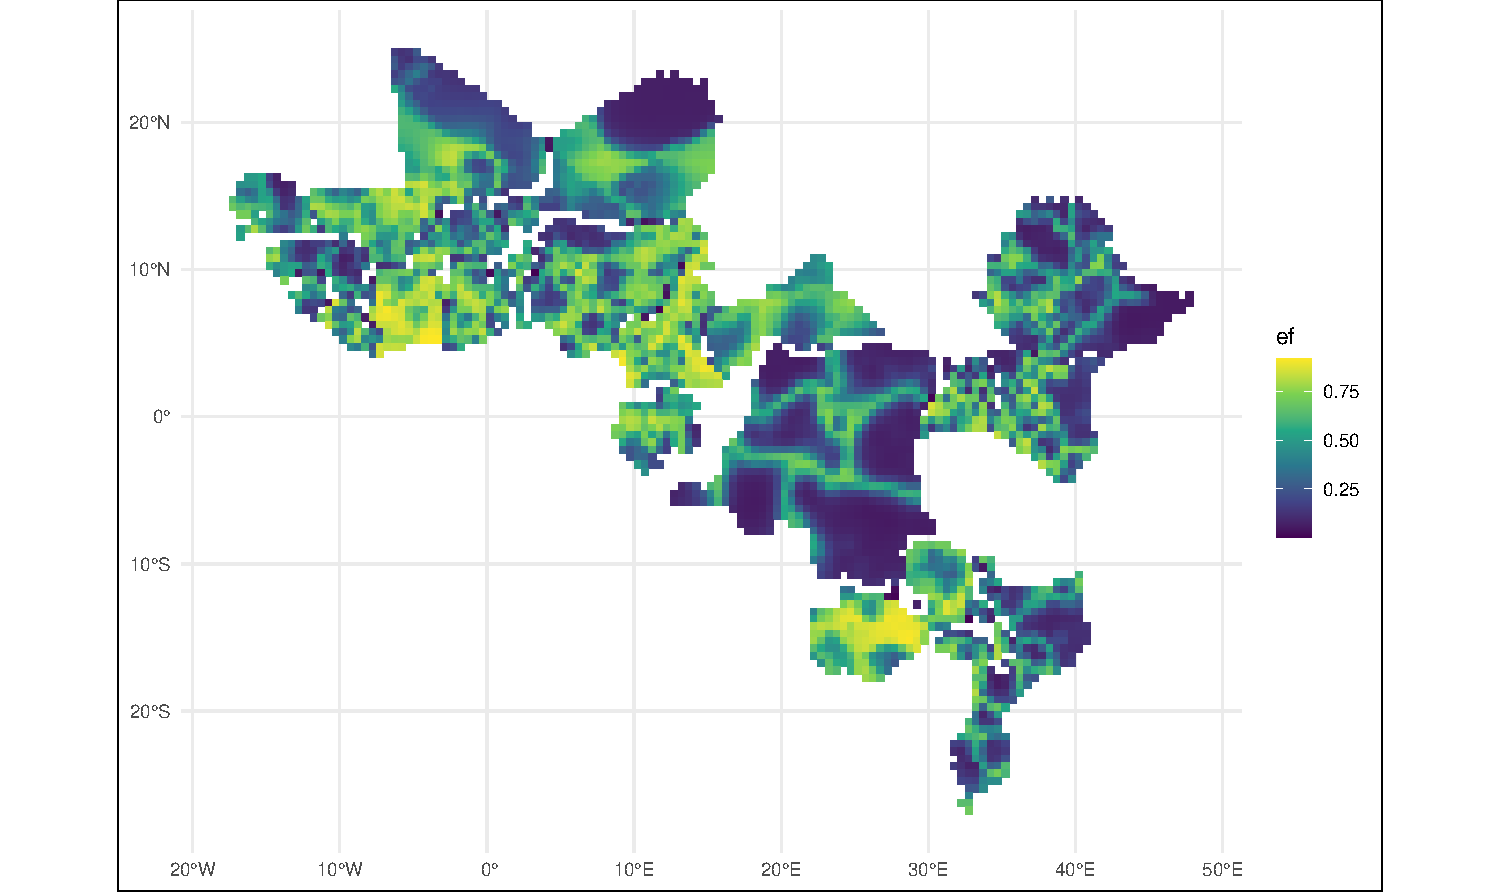
\includegraphics[width=\linewidth]{img/ethplot.pdf}
	\end{figure}

\end{frame}

\begin{frame}{SIDE}

\begin{figure}[htpb]
	\centering
	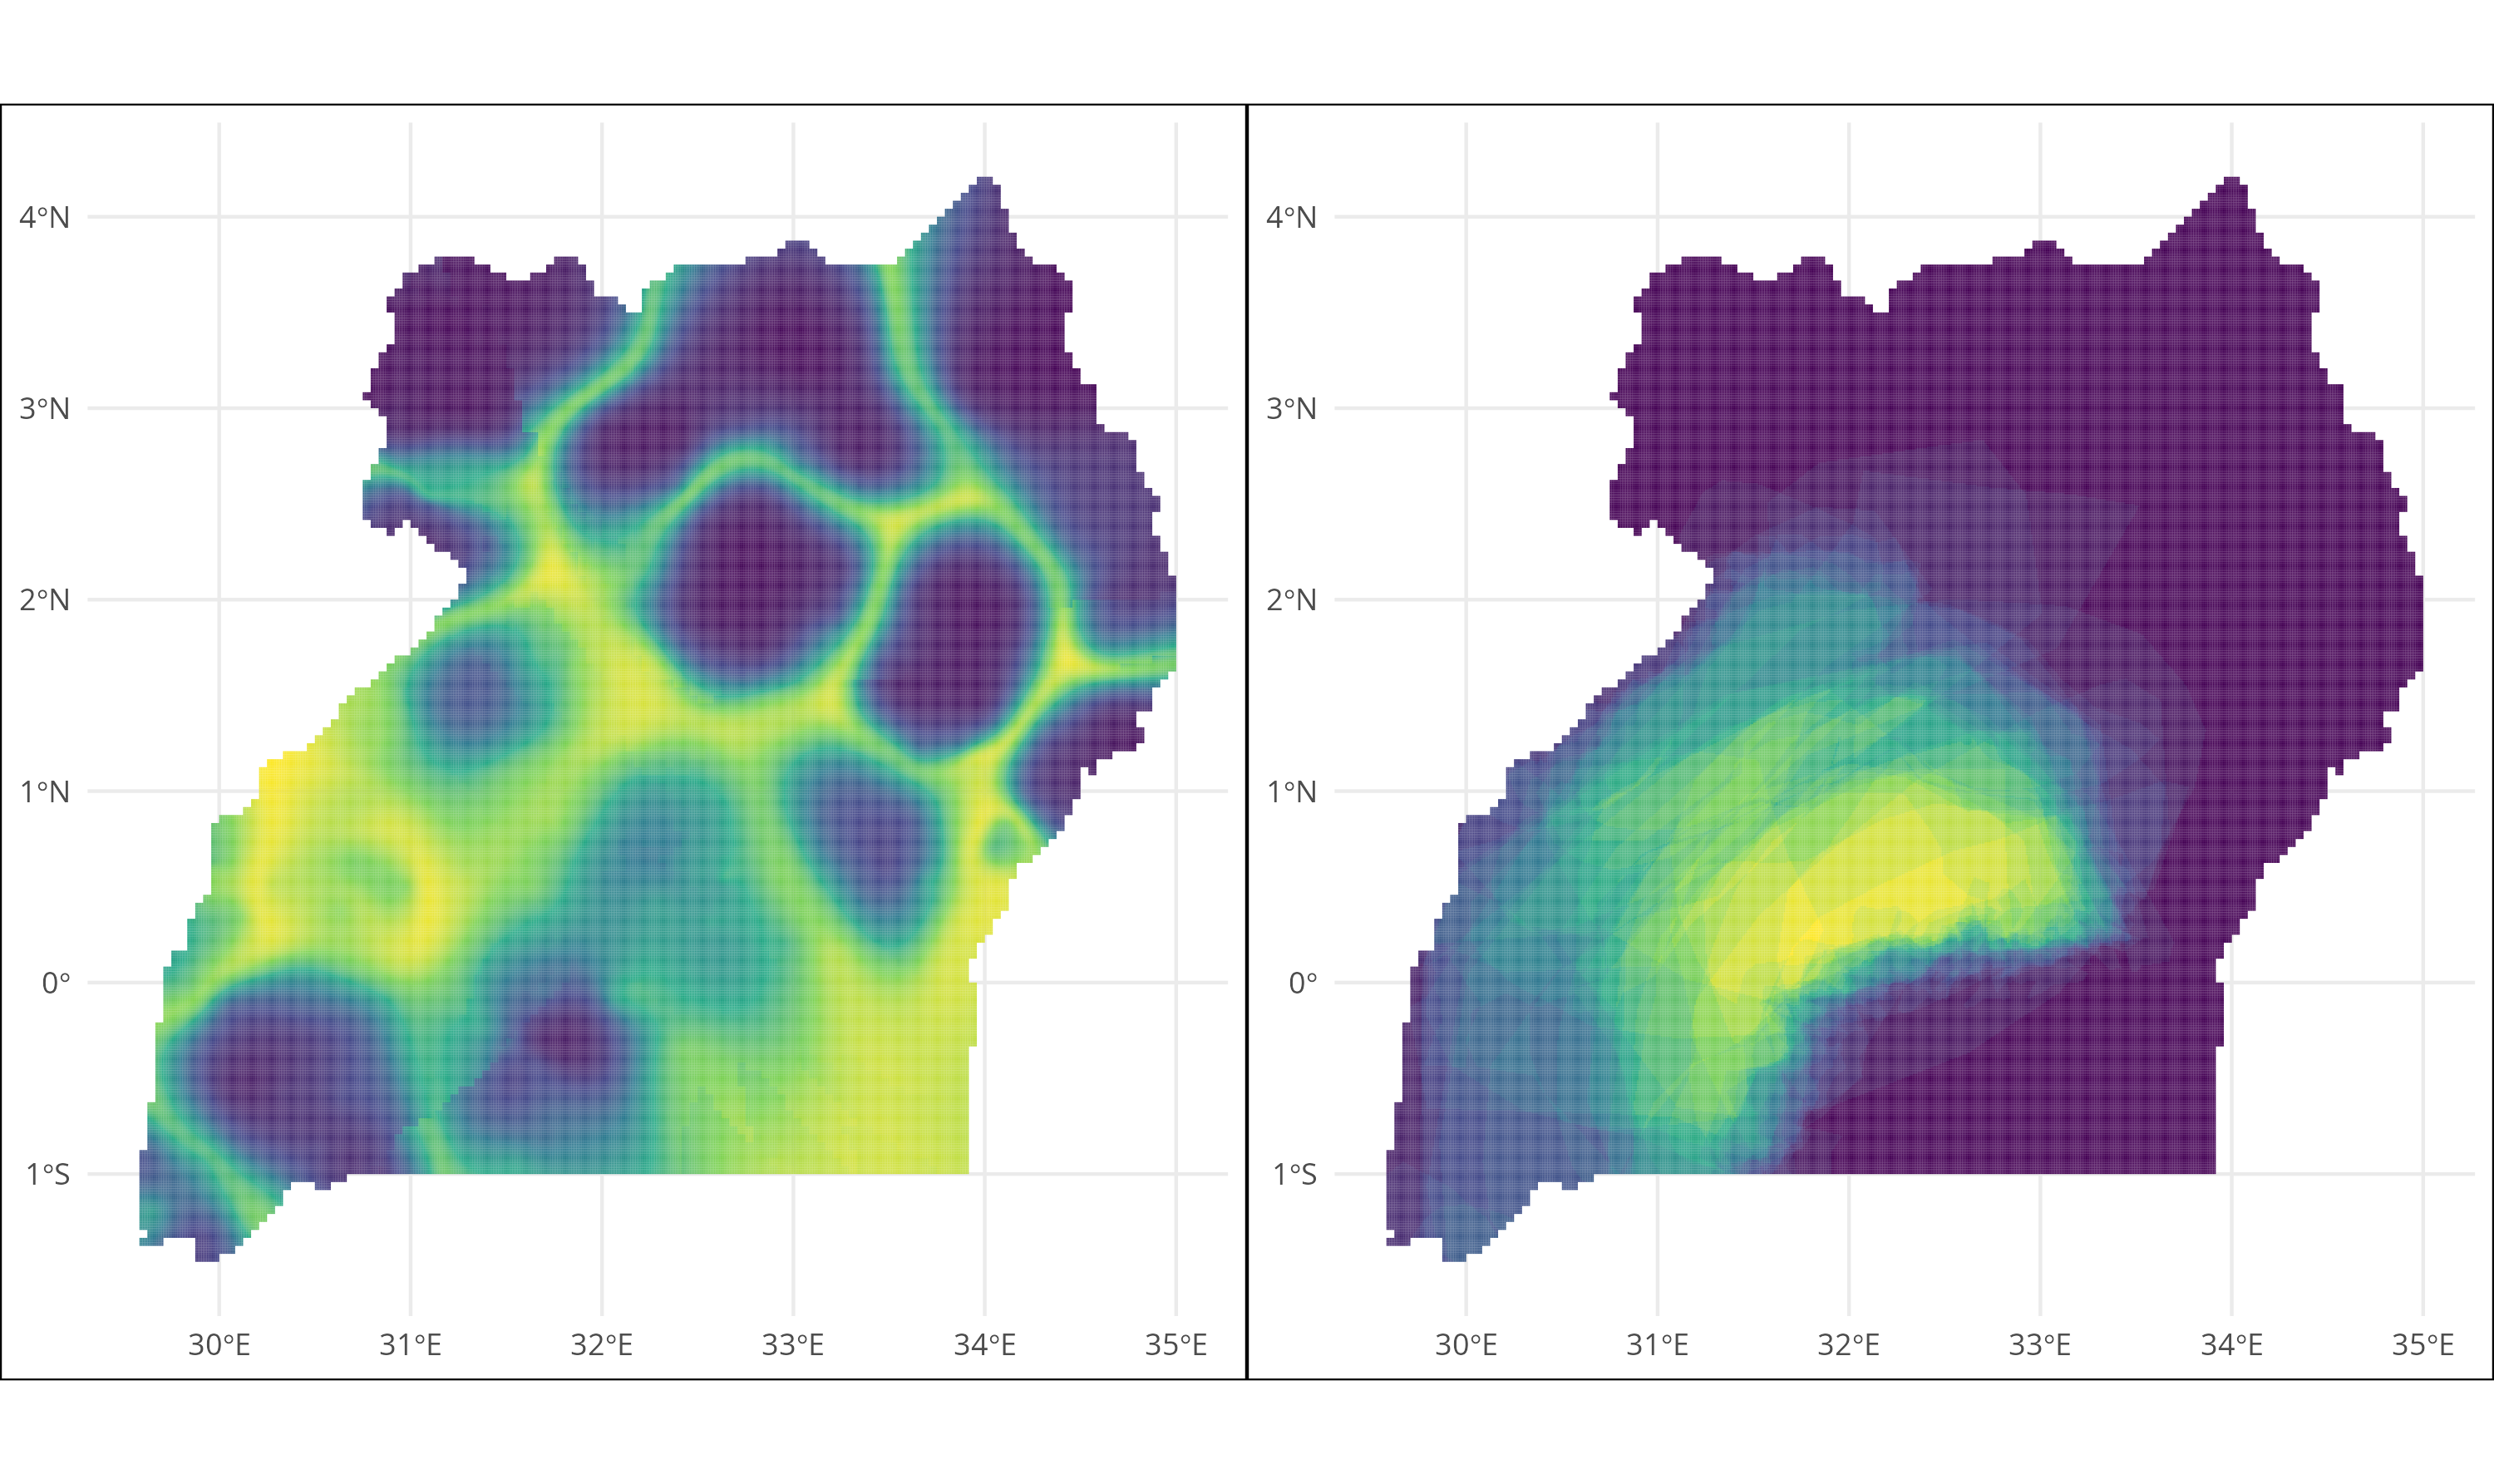
\includegraphics[width=\linewidth]{img/ugaplots.png}
\end{figure}	

\end{frame}

\bibliographystyle{apalike}
\bibliography{../lib.bib}

\end{document}	
